\documentclass[border=3mm]{standalone}
\usepackage{pgfplots}
\pgfplotsset{compat=newest}

% Define custom colors
\definecolor{pastelblue}{rgb}{0.68, 0.78, 0.81}
\definecolor{pastelgreen}{rgb}{0.47, 0.87, 0.47}
\definecolor{pastelyellow}{rgb}{0.99, 0.99, 0.59}
\definecolor{pastelorange}{rgb}{1.0, 0.7, 0.28}
\definecolor{pastelred}{rgb}{1.0, 0.41, 0.38}
\definecolor{pastelpink}{rgb}{1.0, 0.8, 0.86}
\definecolor{pastelteal}{rgb}{0.53, 0.81, 0.92}
\definecolor{pastelmagenta}{rgb}{0.99, 0.6, 0.8}
\definecolor{pastellime}{rgb}{0.8, 1.0, 0.6}
\definecolor{pastelpeach}{rgb}{1.0, 0.9, 0.71}


% Define cycle list macro
\newcommand{\mycyclelist}{
    cycle list={
        {fill=pastelblue},
        {fill=pastelgreen},
        {fill=pastelyellow},
        {fill=pastelorange},
        {fill=pastelred},
        {fill=pastelpink},
        {fill=pastelteal},
        {fill=pastelmagenta},
        {fill=pastellime},
        {fill=pastelpeach},
    }
}

% Define list of x values
\def\myxvalues{{15, 13, 12, 12, 11, 9, 8, 8, 7, 5}}
% Define list of legend labels
\def\mylegendlabels{{"a", "b", "c", "d", "e", "f", "g", "h", "i", "j"}}

\begin{document}
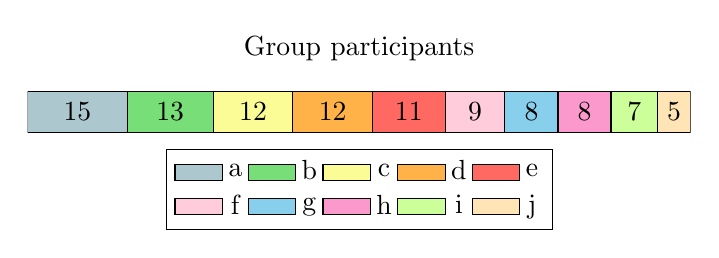
\begin{tikzpicture}
    \begin{axis}[
        xbar stacked,
        bar width=15pt,
        axis lines=none,
        xmin=0,
        xmax=100,
        height=2.2cm,
        width=10cm,
        title={Group participants},
        enlarge y limits={abs=0.1},
        nodes near coords,
        legend style={at={(0.5,-0.1)}, anchor=north, legend columns=5, yshift=-1mm},
        legend image code/.code={
            \draw[#1] (0cm,-0.1cm) rectangle (0.6cm,0.1cm);
        },
        \mycyclelist
    ]
    \pgfplotsinvokeforeach{0,...,9}{
        \pgfmathparse{\mylegendlabels[#1]}
        \edef\tmp{\pgfmathresult}
        \pgfmathparse{\myxvalues[#1]}
        \edef\tmpx{\pgfmathresult}
        \addplot coordinates {(\tmpx,0)};
        \addlegendentryexpanded{\tmp};
    }
    \end{axis}
\end{tikzpicture}
\end{document}